%------------------------------------------------------------------------------
\chapter{Implementation details}
\label{ch:implementation_details}


\section{Application Overview}
\label{sec:application_overview}

Explain how to use the shaders and the commands


\section{\MentalRay Shading Approach}
\label{sec:mental_ray_shading_approach}

How mental ray shoots rays around and what is its paradigm.

\MentalRay approach to solving the rendering equation is based on path tracing, as shown in Figure~\ref{fig:mental_ray_model}, for each pixel in the camera view, an eye ray will be shot in the scene.
On an intersection with an object in the scene, its material shader will be called, this shader will shoot a light ray for each light in the scene, which in effects calls the light shader of the given light.
In order to compute the irradiance at the intersection point, the light shader will probably trace a shadow ray from the light to the intersection point.
Eventually, the material shader will compute the final colour with the information received from the light shader. 

\begin{figure}[htbp!]
\centering
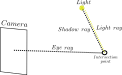
\includegraphics[width=0.8\textwidth]{img/mental_ray_model}
	\caption{\MentalRay simple ray casting example.}
	\label{fig:mental_ray_model}
\end{figure}

Equation~\ref{eq:rte_solution_paper} provides a radiance value for the next march increment, however we want to compute the value at the ray intersection with the volume, i.e. at the ray origin.
So we need to rewrite the equation as

\begin{equation}
\begin{split}
L(\lambda, \x, \omegam) &= e^{\sigma_t(\lambda, \x) \deltax} L(\lambda, x + \Delta\x, \omegam) +  \\
& (1 - e^{\sigma_t(\lambda, \x) \deltax} ) \frac{\sigma_a(\lambda, \x) L_e(\lxo) + \sigma_s(\lambda, \x) L_i(\lxo)}{\sigma_t(\lambda, \x)}.
\end{split}
\end{equation}

\section{Shaders Internals}
\label{sec:shaders_internals}

Talk about things like which parts are written in parallel code, instance support, shader internal memory, sparse data, how the software escalates, memory consumption, Maya integration, spectrum to rgb integration, maybe more details about units for black body radiation and everything that was not explained before

\begin{figure}[htbp!]
\centering
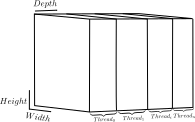
\includegraphics[width=0.8\textwidth]{img/voxel_thread_division}
	\caption{Voxel Dataset division of coefficients computation in threads.}
	\label{fig:voxel_dataset_threaded}
\end{figure}

In order to speed up the render time, all spectrum related computations are integrated to RGB coefficients.
Our spectrum class has a number of samples that can be set a compile time, in general it is set to 30 samples.
However, in certain cases a lower number is used, e.g. when computing the soot absorption coefficients, since we have values for the constants for only four wavelengths, using more than four samples in the spectrum would not improve the results.
The integration is performed first to the XYZ colour space using a Rienmann sum

\begin{equation}
x \approx \frac{1}{\int Y(\lambda) d\lambda} \sum_i X_i c_i,
\end{equation}

where $x$ is the first coefficient in XYZ, $Y(\lambda)$ is the .....s
The conversion from XYZ to RGB is performed using precomputed integrals

\begin{equation}
\begin{bmatrix}
r \\
g \\
b
\end{bmatrix}
 = 
\begin{bmatrix}
\int R(\lambda) X(\lambda) d\lambda & \int R(\lambda) Y(\lambda) d\lambda & \int R(\lambda) Z(\lambda) d\lambda \\
\int G(\lambda) X(\lambda) d\lambda & \int G(\lambda) Y(\lambda) d\lambda & \int G(\lambda) Z(\lambda) d\lambda \\
\int B(\lambda) X(\lambda) d\lambda & \int B(\lambda) Y(\lambda) d\lambda & \int B(\lambda) Z(\lambda) d\lambda
\end{bmatrix}
\begin{bmatrix}
x \\
y \\
z
\end{bmatrix}
\end{equation}

\subsection{Fire Volume Shader}
\label{sec:fire_volume_shader}



\subsection{Fire Light Shader}
\label{sec:fire_light_shader}


\subsection{Voxel Dataset Shader}
\label{sec:voxel_dataset_shader}